\section{Data Decomposition and Computation Mapping}
\label{sec:mapping}

\begin{figure}[t]
  \centering
  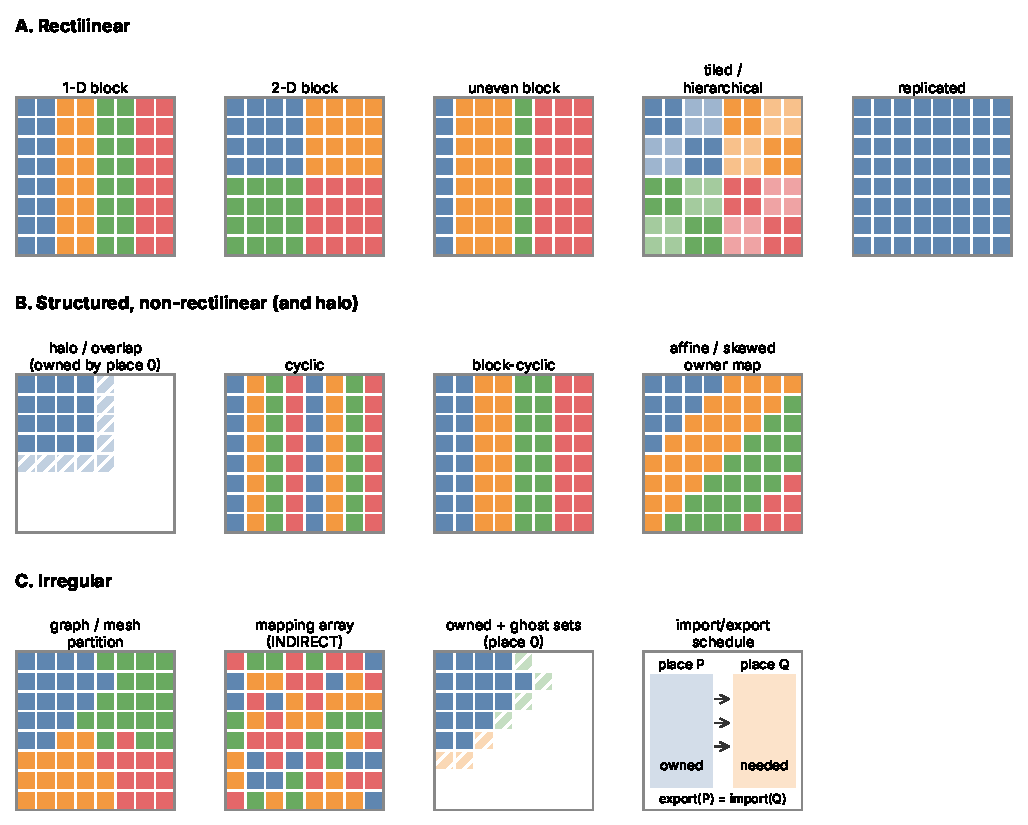
\includegraphics[width=\columnwidth]{decomposition-taxonomy.pdf}
  \caption{Data-decomposition taxonomy (axis~C) drawn as example grids coloured by owning place. Rectilinear forms (A) have closed-form owner functions. Structured non-rectilinear forms (B) need block-cyclic address arithmetic. Irregular forms (C) need a mapping array or graph partition and, usually, run-time schedules. Hatched cells are ghost copies. The examples are illustrative, not drawn from a specific system.}
  \label{fig:decomposition}
\end{figure}

\subsection{Representing ownership (RQ2)}
\ours{Fig.~\ref{fig:decomposition} groups decompositions into rectilinear, structured non-rectilinear and irregular forms.} \fact{Fortran~D and HPF express ownership by aligning arrays to a template and distributing the template over a processor arrangement, using BLOCK, CYCLIC and CYCLIC($k$)~\cite{hpfforum1993spec,loveman1993hpf}.} \fact{Koelbel and Mehrotra's Kali treats distributions as declared properties of arrays over processor arrays, and adds user-defined map functions~\cite{mehrotra1990kali}.} \fact{Vienna Fortran's distribution language includes user-defined distribution functions, alignment with linear expressions, INDIRECT mappings and dynamic redistribution with connect sets~\cite{chapman1991vienna,chapman1992vienna}.} \fact{Chatterjee et al.\ represent the local access sequence of a cyclic(k) distribution with affine alignment as a finite-state machine~\cite{chatterjee1993generating}.} \fact{Gupta and Banerjee choose one distribution per array from weighted constraints~\cite{gupta1992automatic}, and PARADIGM extends this from block to cyclic and block-cyclic distributions by symbolic partitioning~\cite{su1995advanced}.} \fact{Lee's compiler generalises the distribution function and selects layouts across consecutive loops by dynamic programming~\cite{lee1995techniques}.} \fact{Irregular ownership is expressed through a mapping array and partitioner-driven translation in CHAOS, whose partitioner can work from connectivity, coordinates or loads~\cite{ponnusamy1995runtime}.} \fact{Chandra et al.\ add regular and reshaped array distributions as directives on a cache-coherent NUMA multiprocessor, where the data layout is not a message-passing layout~\cite{chandra1997datadist}.} \fact{Modern systems express ownership as per-dimension sharding over a mesh~\cite{xu2021gspmd,mlir2025shard} or as tensor distribution formats~\cite{yadav2022distal}.}

\subsection{Assigning computation (RQ3)}
\fact{Owner-computes assigns an assignment to the owner of its left-hand side. Kali expresses it through on-clauses on doall loops~\cite{mehrotra1990kali}, and the Fortran~D compiler applies it to partition node programs~\cite{hiranandani1991fortrand}.} \fact{Koelbel's closed forms partition the iteration set of a forall loop by the same owners~\cite{koelbel1991regular}.} \fact{PARADIGM partitions iterations and data by symbolic analysis~\cite{su1995advanced} and, in the 1995 overview, combines data and functional parallelism~\cite{banerjee1995paradigm}.} \fact{Legion places tasks and regions through a mapper~\cite{bauer2012legion}, and Sequoia maps tasks to memory levels through a per-machine specification~\cite{fatahalian2006sequoia}.} \fact{ML systems choose among data, operator, pipeline and expert parallelism; Alpa chooses among them per stage with an integer program and dynamic programming~\cite{zheng2022alpa}, and FlexFlow searches per-operator partition configurations~\cite{jia2019flexflow}.}

\subsection{Synthesis}
\infer{Across these systems, the choice of computation mapping follows the choice of data mapping in most cases, and the systems differ in where the choice is made: in the programmer's directives (HPF, Kali), in a closed-form compiler analysis (Koelbel, Chatterjee), in a search over configurations (FlexFlow, Alpa), or in a mapper (Legion). \todo{Compare the expressiveness of HPF's distribution language with GSPMD sharding and DISTAL formats using the specifications \cite{hpfforum1993spec,xu2021gspmd,yadav2022distal}.}}
